\chapter{Data Visualization and Quality Analysis}
\label{chapter:data_study}


\begin{table}[H]
\small
\centering
\caption{Random forest 5-fold cross-validation results with different classification labels}
\label{tab:models}
    \centering
    \begin{tabular}{lcccccc}
        \toprule
        
        Classification Labels                      &   Total Data & Accuracy    & Macro F1    & Precision   & Recall      & MCC.        \\
        
        \addlinespace
        \hline
        \multicolumn{7}{c}{\cellcolor{gray!15}{\textbf{Two Labels}}} \\
        \hline
        \addlinespace
        
        \begin{tabular}[l]{@{}l@{}}Angry, \\ Sad \end{tabular} &         2187 & 92.04$\pm$1.18 & 92.04$\pm$1.18 & 92.05$\pm$1.12 & 92.04$\pm$1.18 & 0.84$\pm$0.02 \\
        \addlinespace
        
        \begin{tabular}[l]{@{}l@{}}Angry, \\ Neutral  \end{tabular} &         2811 & 85.63$\pm$1.18 & 84.42$\pm$1.35 & 86.18$\pm$1.15 & 83.5$\pm$1.4   & 0.7$\pm$0.03 \\
        \addlinespace
        
        \begin{tabular}[l]{@{}l@{}}Sad, \\ Neutral \end{tabular} &         2792 & 78.08$\pm$0.86 & 76.34$\pm$1.08 & 77.3$\pm$0.87  & 75.8$\pm$1.16  & 0.53$\pm$0.02 \\
        \addlinespace
        
        \begin{tabular}[l]{@{}l@{}}Angry$+$Sad, \\ Happy$+$Excited                   \end{tabular} &         2739 & 76.78$\pm$1.89 & 75.32$\pm$2.1  & 76.17$\pm$2.02 & 74.88$\pm$2.12 & 0.51$\pm$0.04  \\
        \addlinespace
        
        \begin{tabular}[l]{@{}l@{}}Sad, \\ Happy$+$Excited \end{tabular} &         2720 & 83.93$\pm$1.66 & 83.27$\pm$1.73 & 83.22$\pm$1.76 & 83.33$\pm$1.72 & 0.67$\pm$0.03 \\
        \addlinespace
        
        \begin{tabular}[l]{@{}l@{}}Neutral, \\ Happy$+$Excited                     \end{tabular} &         3344 & 72.52$\pm$0.75 & 72.32$\pm$0.83 & 72.85$\pm$0.65 & 72.37$\pm$0.79 & 0.45$\pm$0.01 \\
        \addlinespace

        \begin{tabular}[l]{@{}l@{}}Angry$+$Sad, \\ Happy$+$Excited                   \end{tabular} &         3823 & 75.23$\pm$0.77 & 74.22$\pm$0.92 & 75.0$\pm$0.71  & 73.91$\pm$0.94 & 0.49$\pm$0.02 \\
        \addlinespace

        \begin{tabular}[l]{@{}l@{}}Angry$+$Sad,\\Neutral$+$Happy$+$Excited\end{tabular} &         5531 & 73.93$\pm$1.0  & 71.34$\pm$1.13 & 73.43$\pm$1.18 & 70.73$\pm$1.09 & 0.44$\pm$0.02 \\

        \addlinespace
        \hline
        \multicolumn{7}{c}{\cellcolor{gray!15}{\textbf{Three Labels}}} \\
        \hline
        \addlinespace
        
        \begin{tabular}[l]{@{}l@{}}Angry, \\ Happy$+$Excited, \\ Sad                  \end{tabular} &         3823 & 71.96$\pm$1.63 & 72.22$\pm$1.62 & 72.81$\pm$1.56 & 71.95$\pm$1.64 & 0.57$\pm$0.03 \\
        \addlinespace

        \begin{tabular}[l]{@{}l@{}}Angry, \\ Happy$+$Excited, \\ Neutral              \end{tabular} &         4447 & 65.1$\pm$1.56  & 64.77$\pm$1.55 & 66.03$\pm$1.39 & 64.52$\pm$1.65 & 0.48$\pm$0.02 \\
        \addlinespace

        \begin{tabular}[l]{@{}l@{}}Sad, \\ Happy$+$Excited, \\ Neutral                \end{tabular} &         4428 & 64.39$\pm$2.13 & 64.39$\pm$2.11 & 64.91$\pm$2.07 & 64.17$\pm$2.11 & 0.46$\pm$0.03 \\

        \addlinespace
        
        \begin{tabular}[l]{@{}l@{}}Angry, \\ Sad, \\ Neutral                        \end{tabular} &         3895 & 73.81$\pm$1.24 & 73.87$\pm$1.41 & 75.81$\pm$0.83 & 72.7$\pm$1.77  & 0.6$\pm$0.02 \\
        \addlinespace
        
        \begin{tabular}[l]{@{}l@{}}High Arousal, \\ Neutral Arousal, \\ Low Arousal \end{tabular} &         5531 & 68.27$\pm$1.48 & 65.43$\pm$1.89 & 65.73$\pm$1.93 & 65.19$\pm$1.91 & 0.49$\pm$0.02 \\
        \addlinespace
        
        \begin{tabular}[l]{@{}l@{}}High Valence, \\ Neutral Valence, \\ Low Valence \end{tabular} &         5531 & 61.0$\pm$1.11  & 60.1$\pm$1.25  & 60.53$\pm$1.06 & 60.12$\pm$1.22 & 0.41$\pm$0.02 \\

        \addlinespace
        \hline
        \multicolumn{7}{c}{\cellcolor{gray!15}{\textbf{Four Labels}}} \\
        \hline
        \addlinespace
        
        \begin{tabular}[l]{@{}l@{}}Angry, \\ Sad, \\ Neutral, \\ Happy$+$Excited         \end{tabular} &         5531 & 60.26$\pm$0.46 & 60.93$\pm$0.56 & 61.93$\pm$0.62 & 60.49$\pm$0.63 & 0.46$\pm$0.01 \\
        \bottomrule
    \end{tabular}
\end{table}


\begin{table}[H]
\small
\caption{Data duration analysis}
\label{tab:duration}
\centering
    \begin{tabular}{lrrrrrrrr}
        \toprule
        {} & \multicolumn{8}{c}{\textbf{Duration}} \\ \cmidrule{2-9}
        Emotion &    Count &      Mean &       Std &     min &       25\% &      50\% &       75\% &      max \\
        \midrule
        angry   &   1103 &  4.51 & 3.00 &  0.76 &  2.43 &  3.61 &  5.66 &  26.77 \\
        \addlinespace
        excited &   1041 &  4.78 & 3.46 &  0.58 &  2.34 &  3.82 &  6.21 &  34.13 \\
        \addlinespace
        happy   &    595 &  4.34 & 2.71 &  0.89 &  2.39 &  3.56 &  5.80 &  17.22 \\
        \addlinespace
        neutral &   1708 &  3.90 & 2.58 &  0.73 &  2.10 &  3.13 &  4.91 &  20.29 \\
        \addlinespace
        sad     &   1084 &  5.49 & 4.04 &  0.76 &  2.68 &  4.14 &  7.01 &  31.91 \\
        \bottomrule
    \end{tabular}
\end{table}



\begin{table}[H]
\small
\caption{Juries arousal classification analysis}
\label{tab:activation}
\centering
    \begin{tabular}{lrrrrrrrr}
        \toprule
        {} & \multicolumn{8}{c}{\textbf{Arousal}} \\ \cmidrule{2-9}
        Emotion &    Count &      Mean &       Std &     min &       25\% &      50\% &       75\% &      max \\
        \midrule
        angry   &     1103 &  3.63 &  0.67 &  1.5 &  3.0 &  3.5 &  4.0 &  5.0\\         \addlinespace
        excited &     1041 &  3.57 &  0.60 &  2.0 &  3.0 &  3.5 &  4.0 &  5.0\\         \addlinespace
        happy   &      595 &  3.11 &  0.61 &  1.5 &  2.5 &  3.0 &  3.5 &  5.0\\         \addlinespace
        neutral &     1708 &  2.72 &  0.54 &  1.0 &  2.5 &  2.6 &  3.0 &  5.0\\         \addlinespace
        sad     &     1084 &  2.56 &  0.62 &  1.0 &  2.0 &  2.5 &  3.0 &  4.5\\         \addlinespace
        \bottomrule
    \end{tabular}
\end{table}


\begin{table}[H]
\small
\caption{Juries valence classification analysis}
\label{tab:valence}
\centering
    \begin{tabular}{lrrrrrrrr}
        \toprule
        {} & \multicolumn{8}{c}{\textbf{Valence}} \\ \cmidrule{2-9}
        Emotion &    Count &      Mean &       Std &     min &       25\% &      50\% &       75\% &      max \\
        \midrule
        angry   &   1103 &  1.90 &  0.52 &  1.0 &  1.5 &  2.0 &  2.0 &  4.0\\         \addlinespace
        excited &   1041 &  3.94 &  0.62 &  1.5 &  3.5 &  4.0 &  4.5 &  5.5\\         \addlinespace
        happy   &    595 &  3.95 &  0.45 &  2.0 &  4.0 &  4.0 &  4.0 &  5.0\\         \addlinespace
        neutral &   1708 &  2.97 &  0.51 &  1.5 &  2.5 &  3.0 &  3.0 &  5.0\\         \addlinespace
        sad     &   1084 &  2.25 &  0.58 &  1.0 &  2.0 &  2.0 &  2.5 &  4.0\\         \addlinespace
        \bottomrule
    \end{tabular}
\end{table}

\begin{table}[H]
\small
\caption{Juries dominance classification analysis}
\label{tab:dominance}
\centering
    \begin{tabular}{lrrrrrrrr}
        \toprule
        {} & \multicolumn{8}{c}{\textbf{Dominance}} \\ \cmidrule{2-9}
        Emotion &    Count &      Mean &       Std &     min &       25\% &      50\% &       75\% &      max \\
        \midrule
        angry   &    1103 &  3.94 &  0.64 &  1.0 &  3.5 &  4.0 &  4.5 &  5.0\\         \addlinespace
        excited &    1041 &  3.40 &  0.76 &  1.0 &  3.0 &  3.5 &  4.0 &  5.0\\         \addlinespace
        happy   &     595 &  2.92 &  0.65 &  1.5 &  2.5 &  3.0 &  3.5 &  5.0\\         \addlinespace
        neutral &    1708 &  2.83 &  0.60 &  0.5 &  2.5 &  3.0 &  3.0 &  4.5\\         \addlinespace
        sad     &    1084 &  2.82 &  0.81 &  1.0 &  2.3 &  3.0 &  3.5 &  5.0\\         \addlinespace
        \bottomrule
    \end{tabular}
\end{table}


\begin{table}[H]
\small
\caption{Juries dimensional emotion centroids classifications numeric visualization}
\label{tab:dominance}
\centering
    \begin{tabular}{lrrr}
        \toprule
        {} & \multicolumn{3}{c}{\textbf{Centroids}} \\ \cmidrule{2-4}
        Emotion &    Arousal &      Valence &       Dominance \\
        \midrule
        Angry   &    3.63 &  1.90 &  3.94 \\         \addlinespace
        Happy+Excited &  3.40 & 3.94 & 3.23 \\   \addlinespace
        Sad    &   2.56 & 2.25 & 2.82\\         \addlinespace
        Neutral  &  2.72 & 2.97 & 2.83\\         \addlinespace
        \bottomrule
    \end{tabular}
\end{table}


\begin{figure}[H]
  \centering
  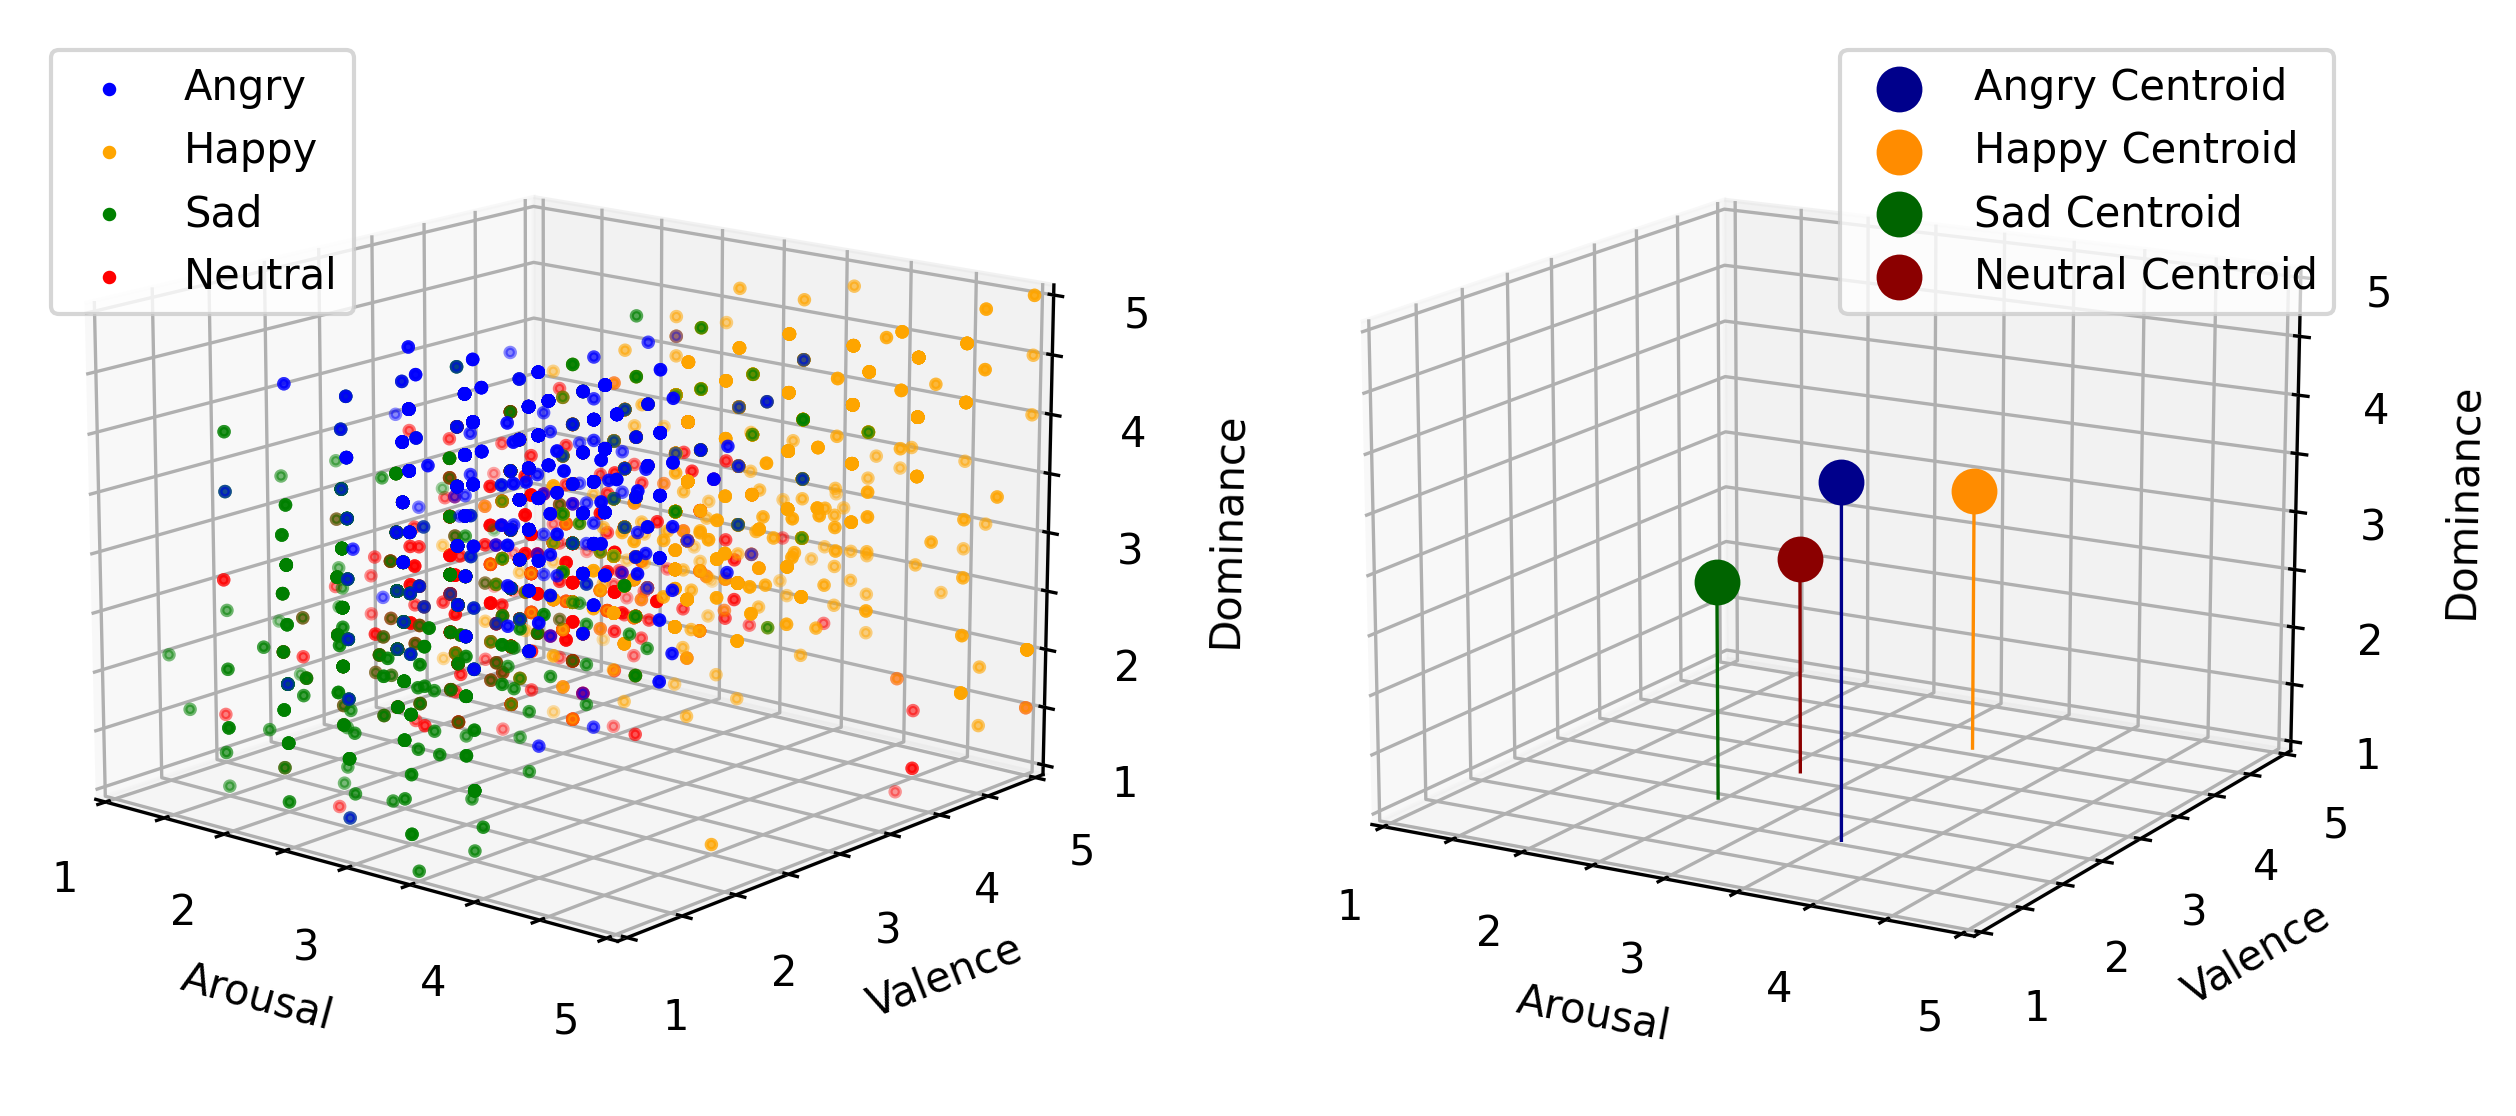
\includegraphics[width=.9\linewidth]{figs/5_data_stratification/primitives_visualization.png}
  \caption{Juries dimensional emotion classifications 3D visualization}
  \label{fig:signalWP}
\end{figure}

\begin{figure}[H]
  \centering
  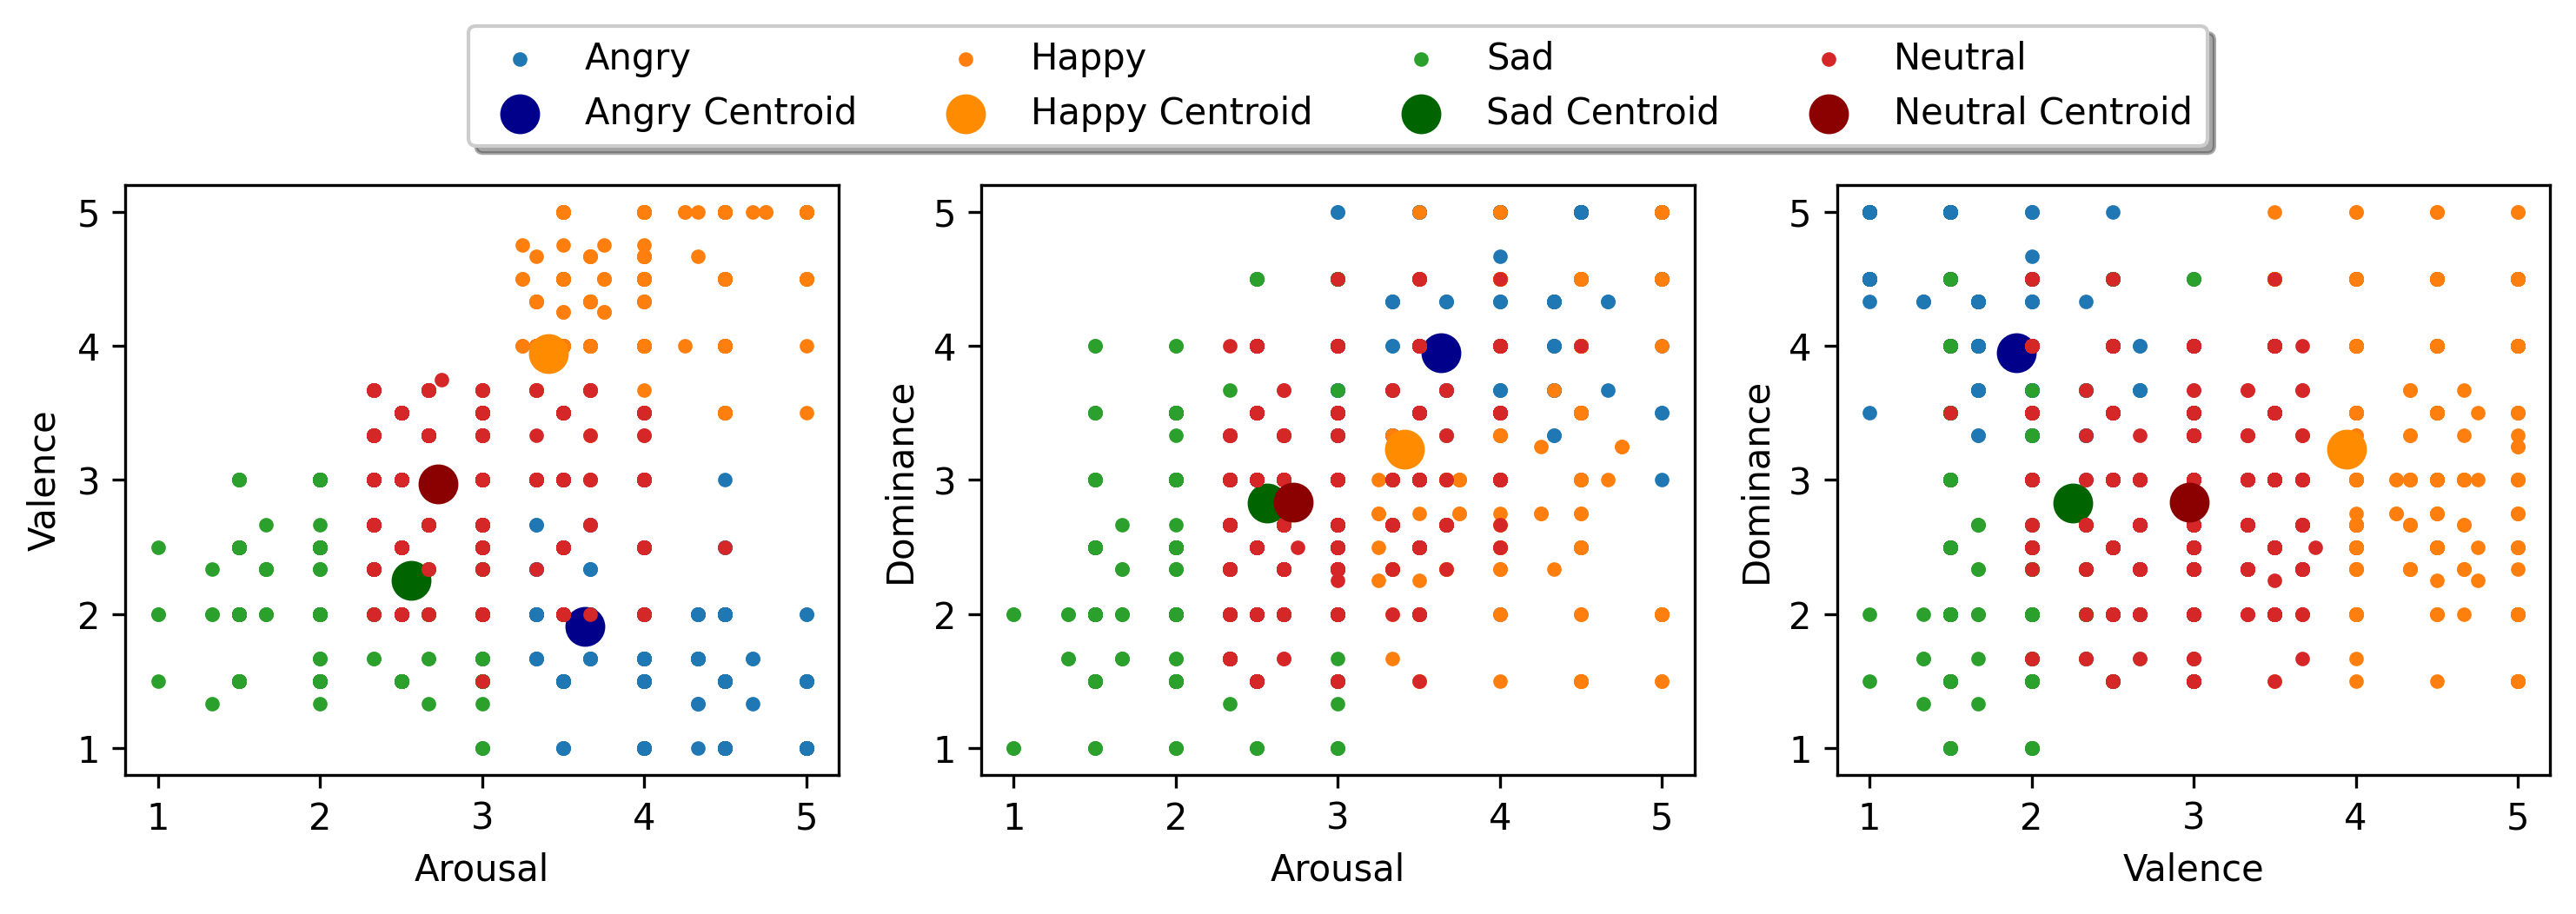
\includegraphics[width=.9\linewidth]{figs/5_data_stratification/primitives_visualization_2d.png}
  \caption{Juries dimensional emotion classifications 2D visualization}
  \label{fig:signalWP}
\end{figure}


CITE CONFLICTS FROM THIS https://ieeexplore.ieee.org/document/9746930:

TODO: NAO MOSTRAR OS CONFLITOS RETIRADOS MAS SIM MOSTRAR OS RANGES MANTIDOS

\begin{table}[H]
\caption{Conflicts between emotion's categories and primitives}
\label{tab:dominance}
\centering
    \begin{tabular}{lrrr}
        \toprule
        {} & \multicolumn{3}{c}{\textbf{Conflicts}} \\ \cmidrule{2-4}
        Emotion Categories &    Arousal &      Valence &       Dominance \\
        
        \addlinespace
        \hline
        \multicolumn{4}{c}{\cellcolor{gray!15}{\textbf{Non-Strict Conflicts}}} \\
        \hline
        \addlinespace
        
        Angry   &    $[1, 2.5]$ & $]3.5, 5]$ & $[1, 2[$ \\         \addlinespace
        Happy+Excited &  $[1, 3[$  & $[1, 3[$ & $[1, 2[$ \\   \addlinespace
        Sad    &    $[3.5, 5]$ & $[3.5, 5]$ & None \\         \addlinespace
        Neutral  &  $[1, 2[$ & $]4, 5]$ & $[1, 1.5[ \cup ]4.5, 5]$\\ 

        \addlinespace
        \hline
        \multicolumn{4}{c}{\cellcolor{gray!15}{\textbf{Strict Conflicts}}} \\
        \hline
        \addlinespace

        Angry   &    $[1, 3]$ &  $[3, 5]$ &  $[1, 2[$ \\         \addlinespace
        Happy+Excited &  $[1, 3]$ & $[1, 3]$ & $[1, 2[$ \\   \addlinespace
        Sad    &   $[4, 5]$ & $[4, 5]$ & None  \\         \addlinespace
        Neutral  &  $[1, 2]$ & $[4, 5]$ & $[1, 2[ \cup ]4, 5]$ \\

        \bottomrule
    \end{tabular}
\end{table}



\begin{figure}[H]
  \centering
  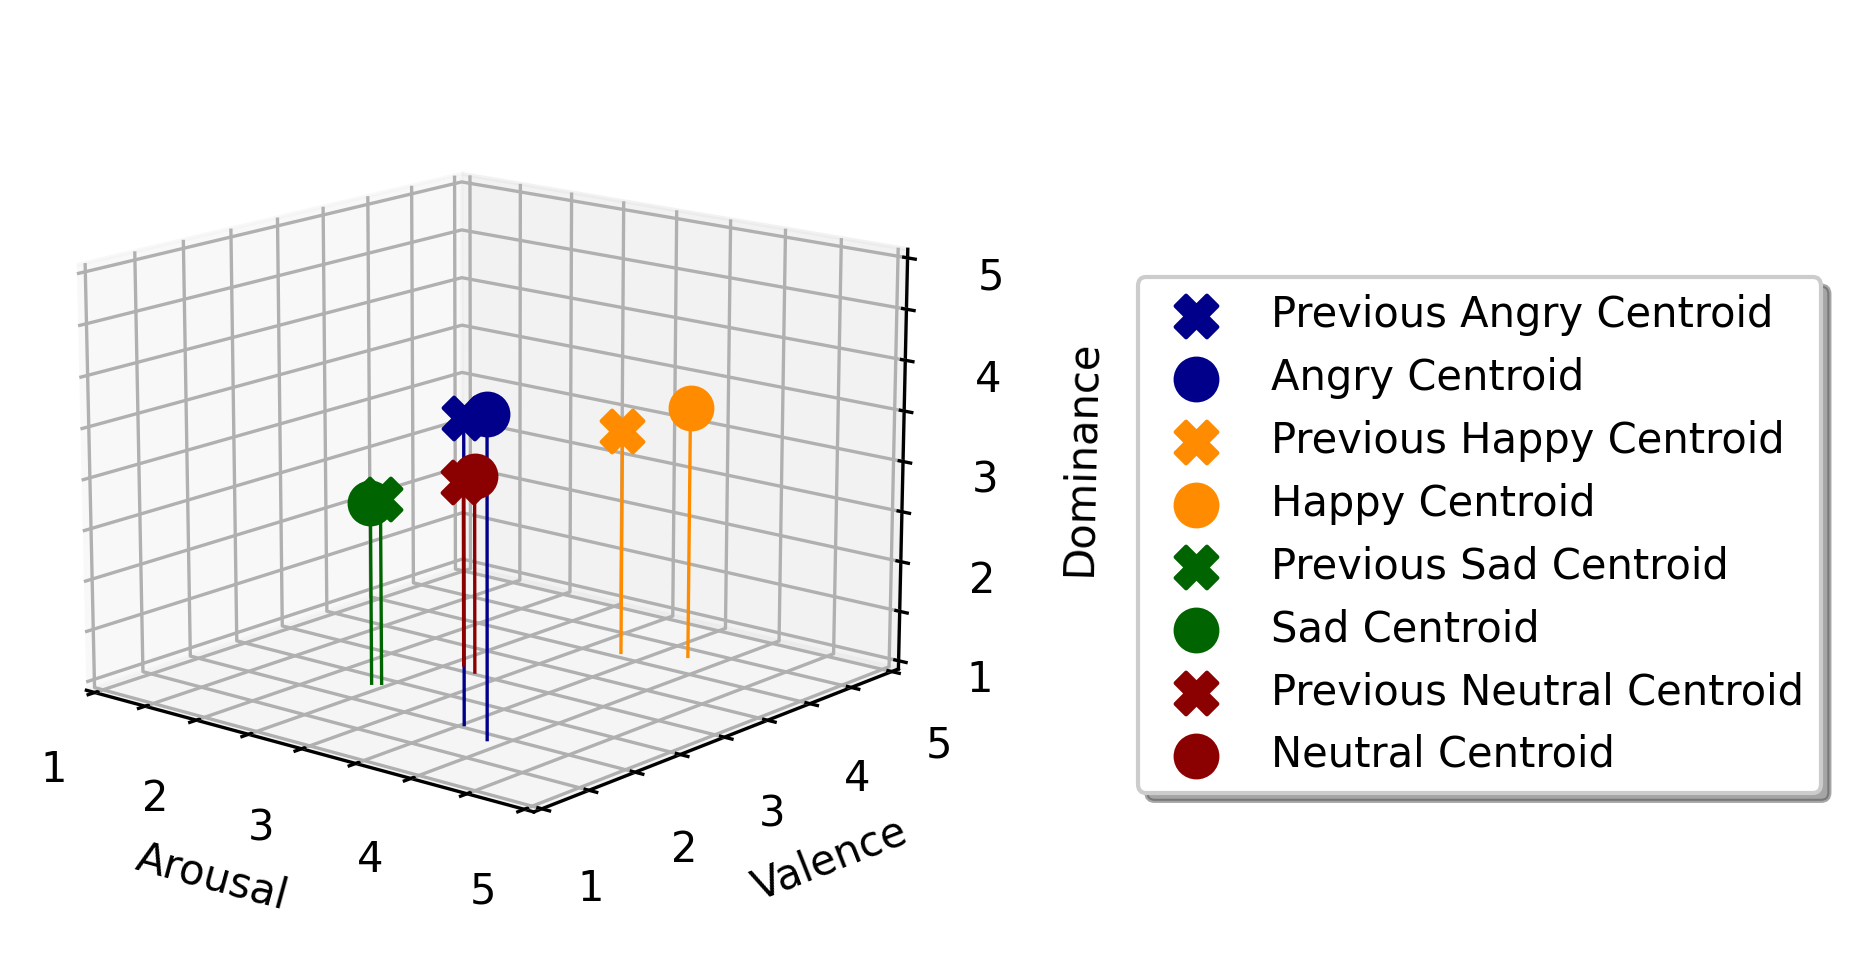
\includegraphics[width=.9\linewidth]{figs/5_data_stratification/strict_conflicts_centroids.png}
  \caption{Data with and without conflicts between emotion's categories and primitives emotion centroids' 3D visualization}
  \label{fig:signalWP}
\end{figure}

\begin{figure}[H]
  \centering
  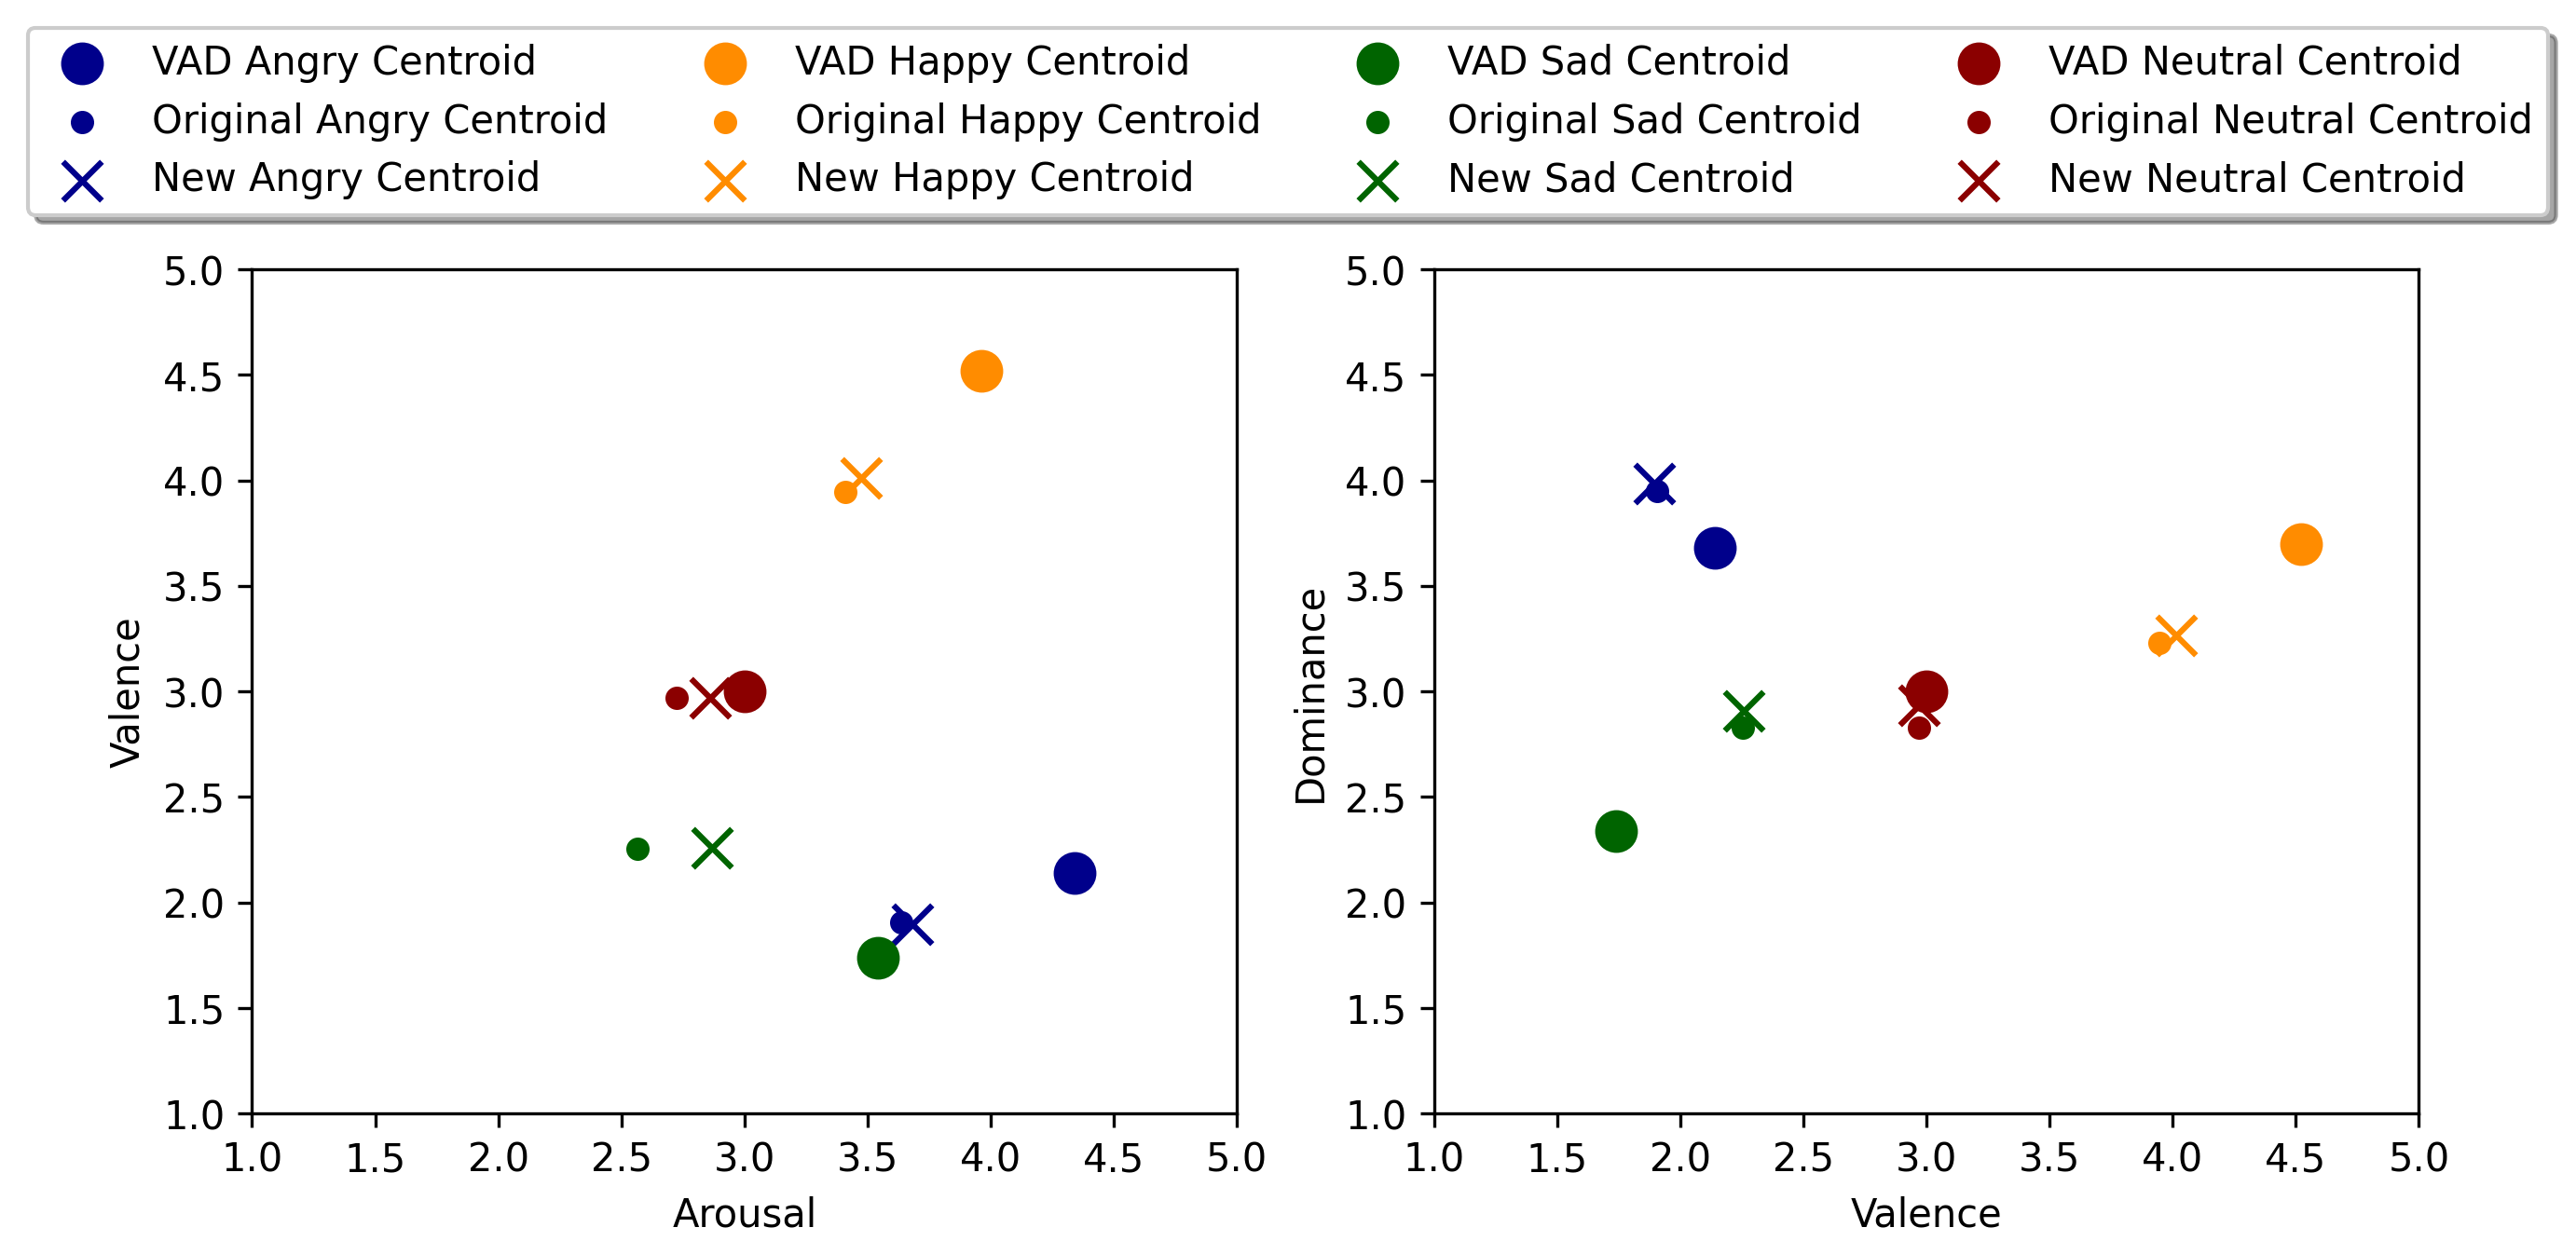
\includegraphics[width=.9\linewidth]{figs/5_data_stratification/strict_conflicts_centroids_2d.png}
  \caption{Data with and without conflicts between emotion's categories and primitives emotion centroids' 2D visualization}
  \label{fig:signalWP}
\end{figure}



\begin{table}[H]
\small
\caption{Results obtained after eliminating emotions based on VAD conflicts with the categorical annotations.}
\label{tab:dominance}
\centering
    \begin{tabular}{lrr}
        \toprule
        Conflicts Removed &    Total Data &  Accuracy  \\
        \midrule
        None & 5531 & 60.26+-0.46 \\         \addlinespace
        
        \hline
        \addlinespace
        
        Non-strict Arousal    &   4955 & 63.37+-1.09 \\         \addlinespace
        Non-strict Valence    &  5382 &  60.46+-0.95 \\   \addlinespace
        Non-strict Dominance   & 5491  & 60.5+-0.93 \\         \addlinespace
        All Non-strict  &  4816 & 65.05+-0.85 \\         \addlinespace
        
        \hline
        \addlinespace
        
        Strict Arousal    &  4222 & 66.79+-1.85 \\         \addlinespace
        Strict Valence    &  5128 &  62.07+-1.77 \\   \addlinespace
        Strict Dominance   & 5432  & 60.53+-1.34 \\         \addlinespace
        All Strict  &  3911 & 69.09+-1.17 \\         \addlinespace
        \bottomrule
    \end{tabular}
\end{table}

TODO: UTILIZAR RANDOMS DADOS PARA CHEGAR AO MSM NUMERO DE DADOS (VARIAS VEZES) PARA VER SE A RAZAO DE MELHORAR DADOS É A QUANTIDADE DE DAODS OU MESMO A MA ANOTACAO